\documentclass[runningheads]{llncs}

\bibliographystyle{splncs04}
\usepackage[utf8]{inputenc}
\usepackage{cmap}
\usepackage{hyperref}
\usepackage{graphicx}
\graphicspath{{./Bilder/}}

\title{History and Evolution of the Browser}
\author{Felix Biedermann, Robert Philippsohn, Jonas Morela}
\institute{University of Stuttgart, Institute for Architecture of Application Systems \\
Universitätsstraße 38, 70569 Stuttgart, Germany}

\begin{document}
\raggedbottom
\maketitle

	\begin{abstract}
		Summary of our paper (70-250 words)
	\end{abstract}

	\section{Introduction}
		\subsection{History and Evolution of the Browser}
		The following deals with history of the browsers and big improvements to the web throught some of these browsers. It continues with showing the fundamental technologies of browsers and features that were implemented later that helped improve the experience of using browsers. And at last this paper will discuss and explore the future of the browsers.
		\subsection{What is a Browser}
		A Browser is an application that interprets HTML documents and data to render them to a Web page making the Web accessable. A browser lets you visit websites and do activities within them like login, view multimedia, link from one site to another, visit one page from another, print, send and receive email, among many other activities. The most common browser software titles on the market are: Microsoft Internet Explorer, Google's Chrome, Mozilla Firefox, Apple's Safari, and Opera. Browser availability depends on the operating system your computer is using (for example: Microsoft Windows, Linux, Ubuntu, Mac OS, among others).

		%Book site 52,https://de.wikipedia.org/wiki/Webbrowser
	\section{History}
		\subsection{The first browsers}
		The first browser for the web was also an invention of the founder of the web, Tim Berners-Lee. The browser was called \textit{WorldWideWeb} and was introduced to the world in the year 1990 [1]. A few years later, in 1994, the Browser was renamed \textit{Nexus}. The browser \textit{WorldWideWeb} was, apart of the fact that it was the first browser, also the first HTML editor.
		To view pictures you had to follow the link of the picture, download it and open it on the computer. Another browser with an diffenrent name but a similar functionality was \textit{Lynx}, which was published 1992 by Thomas Dickey.
		\subsection{First graphical browsers}
		When the Web was published Tim Berners-Lee wanted his invention to succeed. To ensure the success he knew he needed more people to get interested. He needed as many developers as possible to work on web based projects, so there is a constant flow of new content, and he needed the general public to get occupied with the web to make it a long lasting success. For that reason Tim Berners-Lee helped many project that tried to produce new graphical based browsers. In the year 1992 many browser were invented by students as small projects with exactly that goal, were \textit{ViolaWWW} or otherwise called \textit{Viola} was one of the most prominent and \textit{Erwise} was one of the lesser known graphical browsers. But not long after \textit{Viola} came a new competitor. \\This new browser was \textit{Mosaic}.
		\subsection{Mosaic}
		In January 1993 \textit{Mosaic} was published for free and its distribution numbers skyrocketed. Marc Andreessen and Eric Bina, the developers of the \textit{Mosaic} browser, constructed the browser with the intention that a broader audience could use the World Wide Web. That was only possible when the team of NCSA engineers would make their browser accessable for other systems than Unix. Andreessen and Bina, together with some of their NCSA associates, worked on the versions for Mac and PC which came out in late spring of the same year. With this the user numbers of \textit{Mosaic} rose even higher, with 5000 downloads per month. After the graduation of Marc Andreessen and Eric Bina they met James H. Clark, the founde of Silicon Graphics, and discussed how to make the Web commercialisable. That set the starting point for an new Browser called \textit{Netscape}. So Andreessen and Bina left NCSA, with some of their colleagues, in 1994 and settled down in Silicon Valley. After the 2 left the NCSA assigned all commercial rights for \textit{Mosaic} to Spyglass, Inc. Spyglass licensed their technology to many other companies, including Microsoft. In the year 1997 the NCSA discontinued the support for the \textit{Mosaic}, shifting their research focus to other developments projects. The last release for the \textit{Mosaic} browser dates back to August 1997 [2].
		\subsection{Netscape}
		\textit{Netscape} marks the beginning of many important things, that shaped the idea of the browser we know today. The first version of the browser was launched in October 1994 and was programmed by the NCSA team of Andreessen and Bina, that they acquired. In the beginning the team was not sure how to earn money with their browser, but later on their browser marked the end of research-project status of the Web and started the era of the Web of commercial interest and exploitation. The Browser also invented the cookie feature, what lets the browser save data, and the Secure Socket Layer (SSL), what protects the privacy  and integrity of transactions. The first browser was the \textit{Mosaic Netscape} release 0.9. Because of problems with the name the company adapted the name \textit{Netscape Communications} and launched by the end of december the \textit{Netscape Navigator 1.0}, what also solved the problem with the name conflict regarding the NCSA Mosaic browser [3].
		\\Because of the few competetors in the field of browsers, \textit{Netscape} became the most popular browser in a short time. The main income for the company was throught B2B-business and the stock markets. Espacially the stock markets were lucrative, because on the first day (August 9th, 1995) their stock price rose from 28\$ per share to a high of 74.75\$ and at the end of the day they closed off with 58.25\$ [4]. That was a greet sign and it didn't end their; yet. They rose in popularity, until Microsoft started competing in the Web sector. With Microsoft and Netscape Communications the browser wars started [5].
		\subsection{Internet Explorer}
		\textit{Internet Explorer 1.0} (furthemore called IE) was the first attempt of Microsoft on 17 August 1995 to dethrone Netscape as the market leader on the browser territorium. For the first 2 versions of IE, Microsoft used the licensed code of Spyglass Inc. ,from \textit{Mosaic}, as a starting point. The first version that was mostly independently made in the company, would be IE 3.0. It introduced as the first browser ever CSS and it was the first version that did not use the Spyglass source code; only Spyglass technology. It was also the first true competetor for \textit{Netscape}. The following years would become known as the \textbf{Browser Wars} between Netscape and IE, where both parties would improve their browser in a rapid pace. The tides turned with IE 4.0, where Microsoft changed their strategy. Before IE 4.0 their browser was a free browser for the home, like Netscape, but Microsofts' browser was interferior in technology and had to be installed first, before you could use it. But IE 4.0 shipped with all Windows and Macintosh PCs', means the first browser most people interacted with after they bought a new PC was IE and not Netscape [6]. With that IE dethroned Netscape as the most used browser and send Netscape into the depths of nothingness. After the defeat of Netscape the development of Microsofts browser slacked down after the release of IE 6.0 in 2001. But this error made it possible for new competetors to emerge and evolve.
		\subsection{Mozilla Firefox}
		\textit{Mozilla Firefox}, originally called Phoenix or Firebird, is the unoffical offspring of Netscape created in the year 1998. The first version of Firefox, Firefox 1.0, was released on 9 November 2004. Shortly before the release of the first full version Mozilla gained a bunch of new users, because of the warning from the US goverment against the exploit in IE. Firefox and its predecessor were created on the bases of the Netscape source code, which was published on 31 March 1998 in the attempt of Netscape Communications to get more programmers that could improve the code and help defeat Microsoft in the \textbf{Browser Wars}. Unfortunately that was not enough to save Netscape. But it does not mean that Mozilla Firefox was going down with Netscape. The reason behind this was because \textit{Mozilla Firefox} had already its standalone browser, with a big community and enough  programmers  to keep working on the browser [7] [8]. Another reason is the browser was back financially by many investors and the Mozilla Corpration, which was founded as a totally owned branch of the Mozilla Foundation. Nowadays Firefox is still fairly popular browser with 6-8, even while Safari and Google Chrome have a bigger market share.
		\subsection{Opera}
		\textit{Opera} is one of the oldest browsers we have nowadays, next to IE. \textit{Opera 1.0} was first released in the year 1995. It was not as widely used as Netscape or IE, but it gained popularity with time. The intention was to build a fast browser on any system. That is why it was build from scratch and not based on the Mosaic code (like IE and Netscape). But \textit{Opera} gained enough popularity with version 2.1, which was in the on 9 December 1996 and introduced feateures like keyboard shortcuts, zoom and sessions [9].
		\subsection{Safari}
		\textit{Safari} is a browser exclusivly developed for iOS, which was released January 7th, 2003. Initially it was published on Mac desktop systems, later on version 3,4 and 5 it was also published on Windows, but after the 5th version the Windows edition was not further supported. The browser was released for the mobile devices of Apple Inc. in the year 2007. Safari was a pioneer in the browser segment, especially in the early years, but now it is failing to keep with its competitors. Since then the quality decreased from browser version to browser version, compared to its contestant. Currently we have the version 12.1 of the browser for all iOS systems [10].
		\subsection{Google Chrome}
		It was rumored in 2004 that Google was working on a browser, but the development only began in the year 2006. The reason why Google wanted to do their own browser, was because the other options at this time were not that satisfying. The first version was released in 2008 and gained immense popularity. In the year 2012 even surpassed IE in the market share race and since then is dominating the 2nd browser wars and is slowly winning as well. Google also developed an engine for browsers called Chromium, which many browser competitors slowly start using for their own browsers [11].
		\subsection{Tor Browser}
		The \textit{Tor Browser} is a browser with one goal: internet user should have access to an uncensored web, without being tracked by anyone. Tor stands for "The Onion Routing", the technology that fuels the \textit{Tor Browser}. October 2002 the Tor network was deployed but no browser to access it, so people without technology experience were not able to access the network. The work on the \textit{Tor Browser} started in 2008 to help those without the knowledge to do so before. The browser was later on tool to many political movements, like the Arabic Spring in 2010, and popularity after Snowden's revelations in 2013. [12]
		\subsection{Timeline of all browsers}	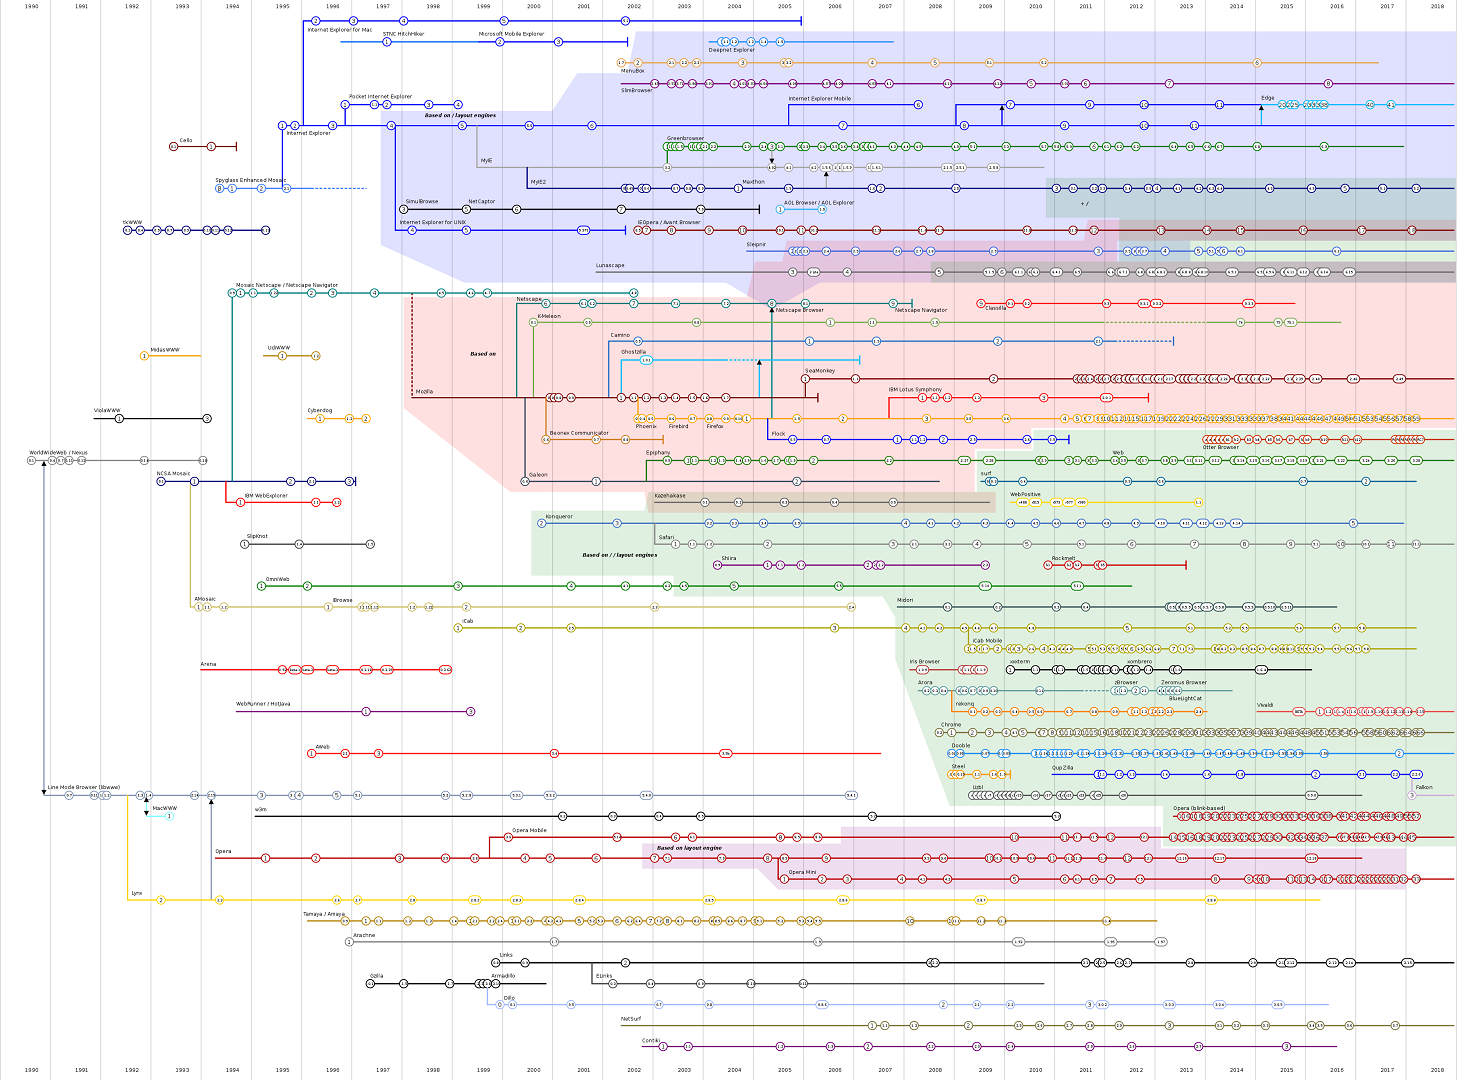
\includegraphics[scale=0.7]{TimelineOfWebBrowsers.png}
			\begin{center}
				\textit{\textbf{A timeline of all browsers and browser versions ever made. [13]}}\\
			\end{center}

		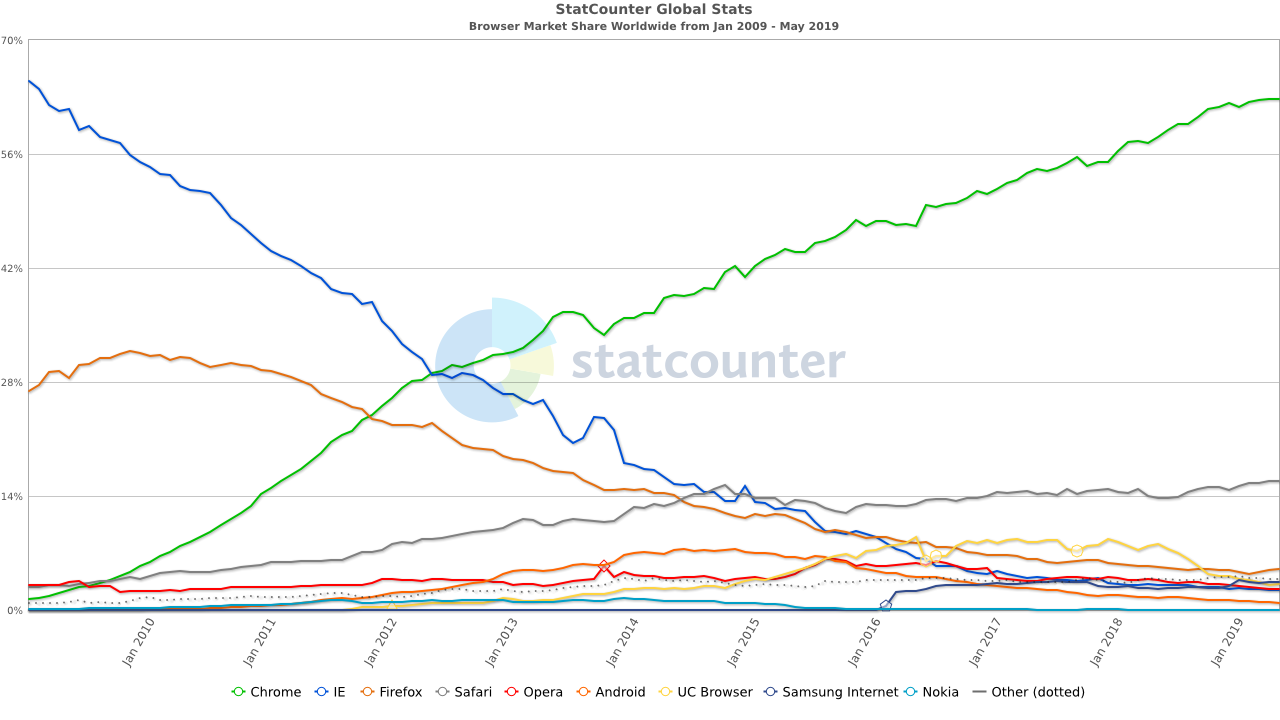
\includegraphics[scale=0.31]{WebBrowserMarketShare.png}
		\begin{center}
			\textit{\textbf{A market share timeline from 2009 to 2019 for the most used browsers.[14]}}
		\end{center}
		
		\subsection{Browser nowadays}
		Today Google Chrome dominates the browser market, with roughly 60\%-65\%. Next up is Mozilla Firefox according to the data, with 5\%-8\%. After that we have Internet Explorer and its successor Microsoft Edge, both with around 5\%-7\%. Every other browser has less than 5\% market share. Another fact to mention is that most browser use Chromium, the browser engine of Google, including Opera, Microsoft Edge and other browsers. The only widely used browsers that don't use Chromium are Mozilla Firefox and Safari.\\
		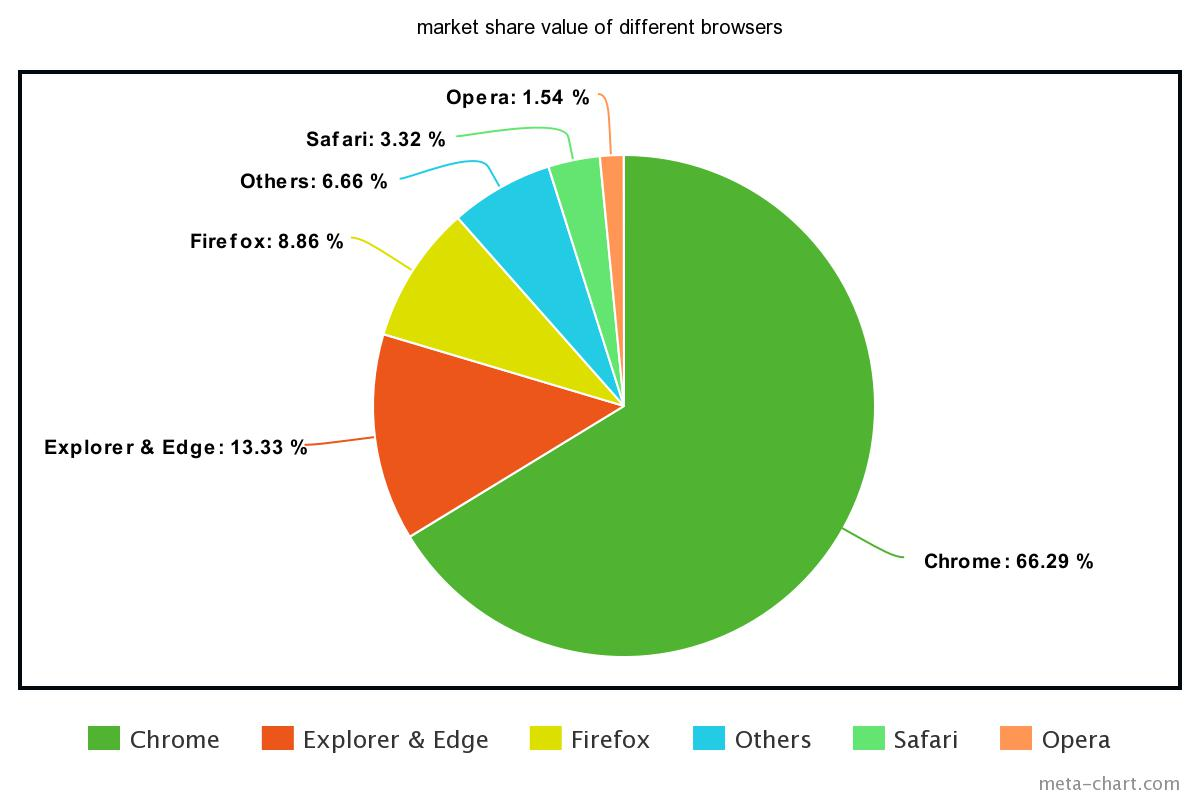
\includegraphics[scale=0.3]{meta-chart.jpeg}\\
		\begin{center}
			\textit{\textbf{The market share value of the different browsers from June 2019. [15]}}
		\end{center}
		
	\section{Evolution}
		\subsection{The meaning of Evolution}
		With every new browser and browser version being released features and improvment have been added. Browsers became more secure, user and developer friendly, and more efficient. These were implemented because of new technologies, bugs being discovered and in trying to run out the competition. If you add all of the changes to a timeline you can overview the Evolution of the browser.
		%Evolution of the browser Website pic
		\subsection{How Patches influenced Browsers}
			\begin{quote}``I call such changes patches, as they are attempts to fix the original design of the web'' Marco Aiello The Web was Done by Amateurs S. 65 \end{quote}
		By changing the Web, patches also influenced browsers when they were introduced. In this chapter we will have a short summary of what these patches were and how browsers evolved and adpaped through these changes.
			\subsubsection{Cookies}
			\leavevmode\newline
			Like mentioned before Cookies were introduced with Netscape in 1994 for websites to be able to save data to be remembered for processes on the clients side. The original idea The webbrowser is being used by the server of the website to save textinformation on the Computer of the client. These have made it possible to save login and shopping cart informations but also made Webtracking possible. Later they received critizism for being able to damage the users privacy and threadening security when surfing the web. Under the EU's GDPR Law websites are now forced now ask and inform users about saving data in their Browser.
			%http cookie wikipedia english/german and Book
			\subsubsection{SSL}
			\leavevmode\newline
			SSL is the short form for Secure Sockets Layers, which was an introduction of an security system in the Web. One could say that SSL is an application layer based security protocol but that is not entirely true. It actually is used in the session layer which is above the transport layer and beneath the application layer [16]. It was introduced by Netscape and shaped the security protocols we use nowadays. SSL had many flaws that were corrected by its successors TSL, thats why the latest version was deprecated in the year 2015.
			
			\subsubsection{Java}
			\leavevmode\newline
			In the year 1995, Sun Microsystems published the object-oriented programming language \textit{Java}, inspired by James Gosling. \textit{Java}, formerly called Oak, is able to run on every computer. This is made possible by the Java Virtual Machine, which takes the standard bytecode instructions of the Java program and interpretes it. The only problem is that the JVM is not uniformly implemented across all hardware vendors. The combination of Java and the Web is only possible if the JVM is available to browser on the client side. The Java code is send with the the Web page, where this code is known as Applet. When the browser hits the point where the code should be run, it starts an instance of the JVM and gives it the bytecodes for the execution. [17]
			\subsubsection{JavaScript Engines} \leavevmode\newline
			While it would have been possible to couple the handling of JavaScript to the browser engine, every major browser uses a dedicated script engine. This is due to the fact, that JavaScript, while originally created for use in web browsers, is now also used elsewhere. In the web browser these two engines interact with each other through the shared DOM data structure.
			The first JS engines started with bare interpreters and evolved to full engines with several additional features. The first JavaScript engine was developed by Brendan Eich, co-founder of the Mozilla project, in 1995 for \textit{Netscape}. It was a bare interpreter for the language he was inventing at this time. The first modern JavaScript engine was Googles V8 engine, created for Chrome in 2008. The key innovations was just-in-time compilation, boosting performance significantly. As a result other browser vendors had to overhaul their interpreters to develop into full JavaScript engines. This lead to the development of the Nitro engine for Apples \textit{Safari} browser. Mozilla used portions of Nitro to improve SpiderMonkey, which resulted from Brendan Eichs original JavaScript interpreter. Opera replaced their interpreter with their Carakan engine, also boosting performance significantly.
			Since 2017 all major browser have added support for WebAssembly to their JavaScript engines. This gives the ability to execute pre-compiled scripts for performance-critical parts of the web page. The code is executed in the same sandbox as the regular JS code.
			
		\subsection{Basic Technological Changes}
			\subsubsection{HTTP}
			\leavevmode\newline
			\textit{HTTP} stands for HyperText Transfer Protocol. It is an aplication-level, request-reply protocol which is typically transported by a lower-level protocol, like TCP. It works like follows: if the client requests a ressource, the server replys with information and sometime even the ressource itself [17]. Today one differenciates between HTTP and HTTPs, where HTTPs means HyperText Transfer Protocol secure because the HTTP is acompanied by a SSL encryption.
			\subsubsection{HTML}
			\leavevmode\newline
			\textit{HTML} is the abbreviation for HyperText Markup Language. Tim Berners-Lee made this textual format for annotating plain text with informations part of his original Web proposal, and created the first editor and at the same time the first browser around HTML. The first proposal for HTML is dated back to 1993, but today HTML 5 exists; which was standardized in 2014. [17]
			\subsubsection{URL}
			\leavevmode\newline
			\textit{URL} is the short form for Uniform Resource Locator. The \textit{URL} gives the address where specific ressources are located in the Internet and the protocol to access it. The URL contains furthermore the port number to access the address, the location of the resource in the server and a fragment identifier [18]. The \textit{URL} is also one part of the original proposal of the Web from Tim Berners-Lee. 
			%TODO: Move to another location?
			\subsubsection{Browser Engines}
			\leavevmode\newline
			The browser engine, also called "layout engine" or "rendering engine", is the core component of most major web browsers. The job of a browser engine ist the transformation of HTML files and other required resources to an interactive web page. While it is possible to separate the engine for the layout and the rendering of the page, in practice they are mostly coupled and not seperated. The browser engine is also responsible for enforcing the web pages security policy and creating the DOM data structure used in scripts. It is also responsible for handling hyperlinks and web forms.
			Browser engines may also be reused in other application. An email client, for example, may use such an engine for rendering HTML emails. Another example is the "Electron Framework", which uses the engine of \textit{Google Chrome}, used to create many applications. The layout to be rendered is specified by the CSS file of the web page. There are several different browser engine implementations and the most major web browsers use their own browser engine. Examples are Gecko by Mozilla, WebKit by Apple and Blink by Google. Microsoft used to have their own browser engines Trident and EdgeHTML, but use Googles Blink browser engine now.
		\subsection{Features}
			\subsubsection{History}
			\subsubsection{Incognito mode}
			\leavevmode\newline
			Private browsing was first added in 2005 by \textit{Safari} on Mac. The feature has since been adapted by many other browsers so that most modern browser have some form of private browsing.
			\subsubsection{Bookmarks}
			\leavevmode\newline
			Bookmarks were a quite early feature and have been included since \textit{Mosaic} in 1993, altough called hotlists back then. Newer browsers have expanded the feature of bookmarks. \textit{Firefox} for example, introduced so called "Live Bookmarks" which are essentially bookmarks provided as RSS feed.
			\subsubsection{Browser Extensions}
			\leavevmode\newline
			As the first major browser, \textit{Internet Explorer} introduced browser extensions with Version 5 in 1999. The other major browsers also added extensions over the years with Firefox in 2004, Opera in 2009 and Google Chrome and Safari in 2010. Nowadays most browsers support extensions to customize the user experience.
			\subsubsection{Tabs}
			\leavevmode\newline
			The first web browsers did not have tabs as we know them from most modern browsers. While many may consider \textit{Opera} to be the browser to introduce tabbed browsing, \textit{Opera} had a  \textit{Multiple Document Interface} instead. This may seem similar but is substantial different to a \textit{Tabbed Document Interface}. The actual first browser supporting tabs was the \textit{Internet Explorer} Shell "NetCaptor", first released in 1997. The browser to mainstream browser tabs was however Firefox or more specifically its predecessor \textit{Phoenix}.
			\subsubsection{Browser Chache}
			\leavevmode\newline

	%Prof meinte guter Fokus.
	\section{Future of the Browser}
	Nowadays there are already many ways to interact with a browser which seem rather futuristic. You can controll via voice, by hand gestures and even by just looking with your eyes. You are not just having you browser on your Computer but also on your phone, your watch and floating in the air infront of you.
	%Pic of alexa, firefox vr, eye study
		\subsection{Browsers becoming operating systems}
		One of Alan Kay's main crizisms about the Web is the absence of an computational abilty for the browser. His vision is for them to be like  mini-operating systems and being able to execute localy. So it is possible for example if you want to learn an programming language you can just write code on the website and execute it on your computer. The patches where already steps into the right direction. Another part is to make website be like applications and with web applications like google docs or Microsoft office home the browser is going towards that vision. These make it possible to create, send and receive content like documents or tables while other people can access them simultaneously. It is for sure that more applications like these will be released.

		An good example for a website supporting Alan Kay's vision is lively-web.org
		%Screenshot
		Everything that is displayed on the website is an object and can be changed, moved or overwritten and gives immediate feedback to the user. Every textfield is able to execute Javascript. You can create your own website or application and are able to edit and download it from everywhere.
		%TODO How does it work?
		%Before after Picture
		%Book,
		\subsection{New technologies}
			\subsubsection{WebVR Browsers}
				\leavevmode\newline
				Virtual Reality Browsers are making it possible to access the Web with VR-Glasses. To navigate the voice or a virtual keyboard can be used. The Browsers makes it possible to watch 360 degrees videos or pictures. Developers are able to create WebVR Applications themself and put them on the web just like a website. Vr-Browsers like Firefox Reality or Supermedium Browser allow to display websites not like a 2D Sheet but rather like a 3D environment without having to download content. These evironments can also be experiences, see second picture, games or creative activities like 3D painting.
			\begin{center}
				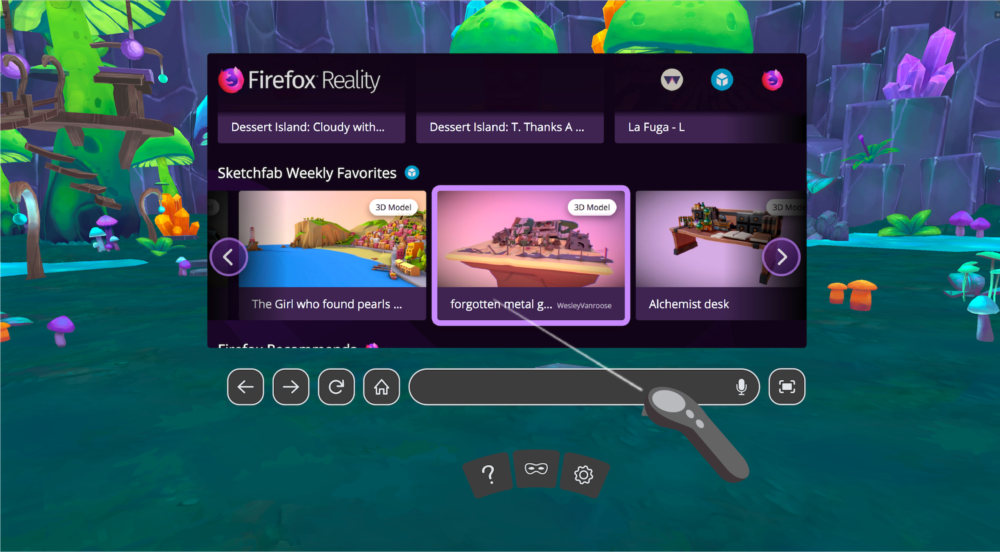
\includegraphics[scale=0.35]{Firefox_Reality.png}
				[19]	Firefox Reality
				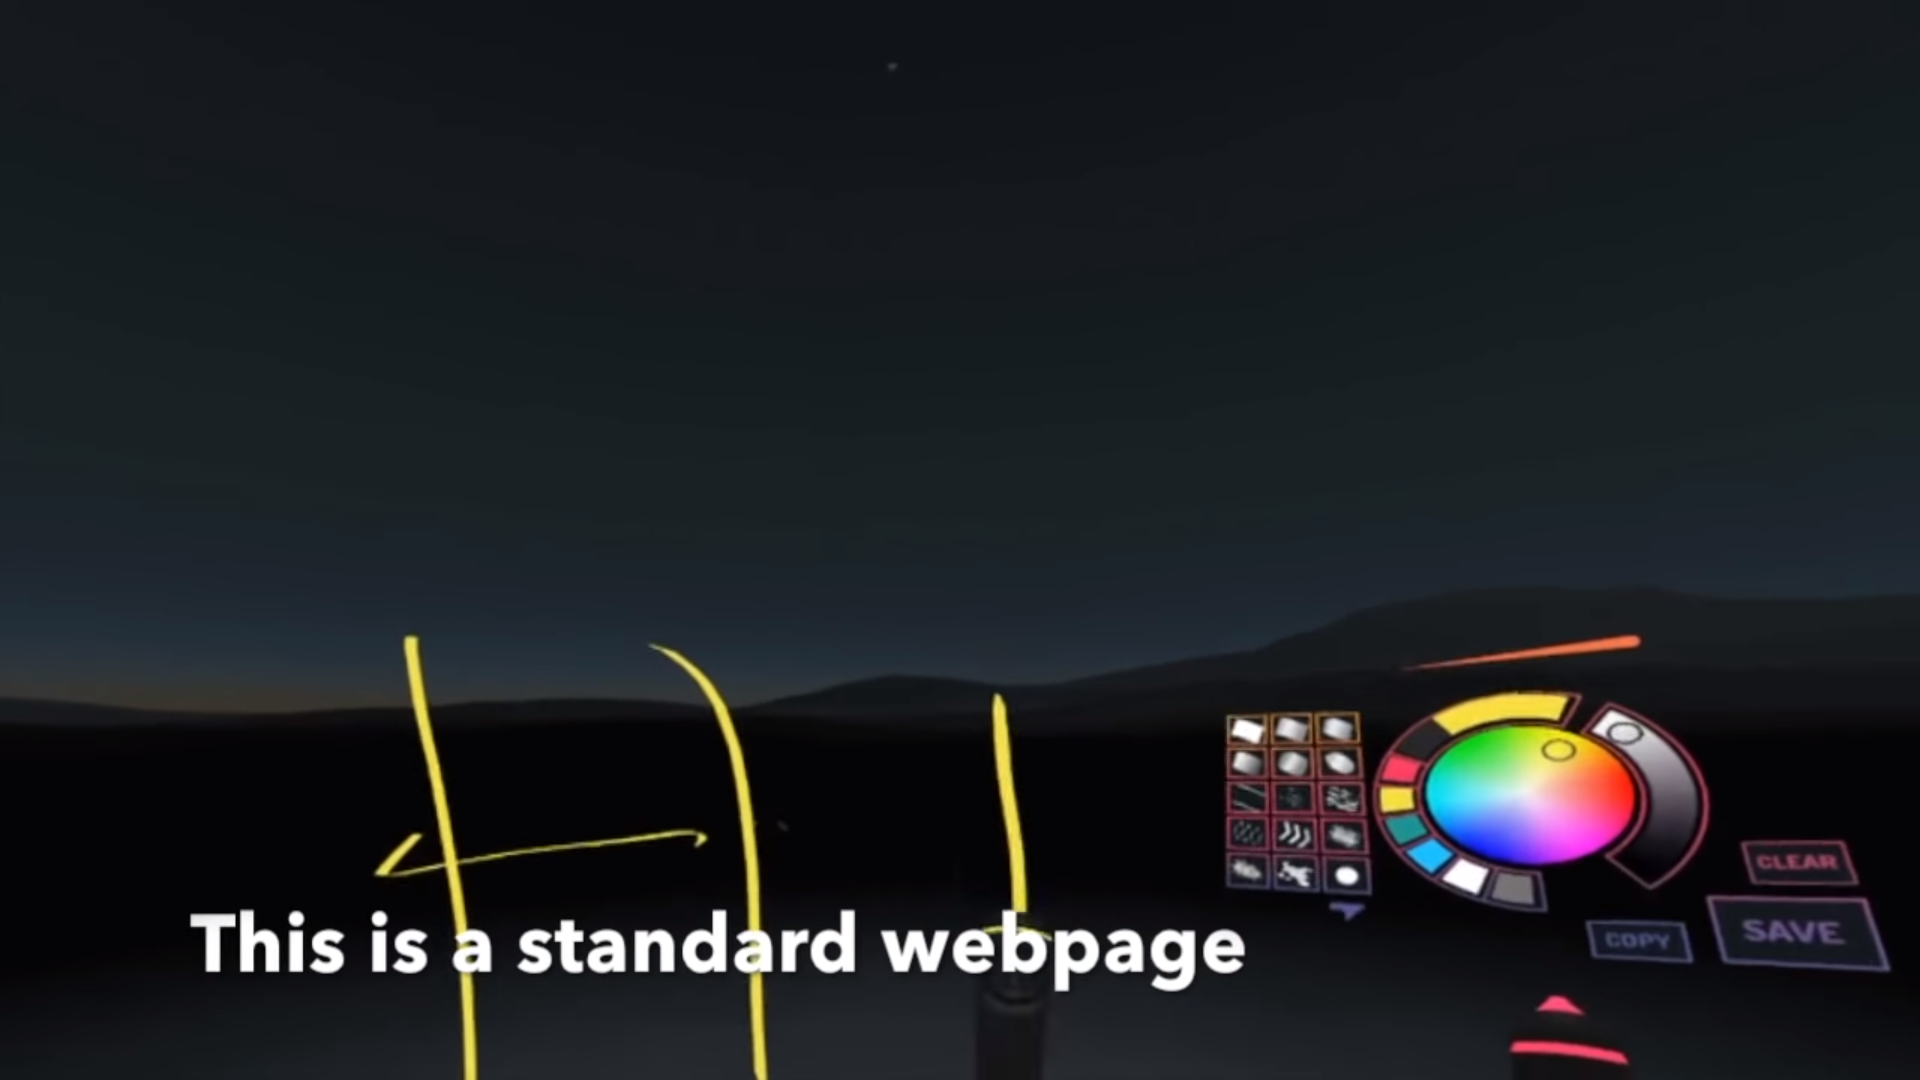
\includegraphics[scale=0.35]{Supermedium.png}
				[20] Supermedium Browser
			\end{center}
			\subsubsection{AR Browsers}
				\leavevmode\newline
				Just like normal Browsers is an Air Browser an applciation. The difference is that AR Browsers are for phone or tablet use only. Their purpose is to display additional informations on a camera screen. These Informations can be 2D markers or 3D objects for example.Just like most of VR Browsers they also rely on content creators. 
				%https://www.augmented-minds.com/de/erweiterte-realitaet/ar-app-und-ar-browser/
			\subsubsection{Quantum computing}
			\leavevmode\newline
				Another big topic of these times is quantum computing. Quantum computers would make it significantly easier to decrypt keys for the secure transport of data between the browser and servers. Thats why since a couple of years institutes around the world are looking for algorithms that are post-quantum secure. Meaning that their generated keys can withstand the decryption of an quantum computer longer than algorithms nowadays like RSA. Browsers will need to adapt to these changes in order to asure security for it's customers and stay competitve on the market. 
				%TODO 	https://www.f5.com/labs/articles/threat-intelligence/how-quantum-computing-will-change-browser-encryption
		\subsection{Next for Browsers}
			Since the introduction of the browser a little and a lot has changed. It gained on speed, performance, security and usabilty. These attributes with grow in the future as well for sure. 
			Opera created an concept for how they imagine user friendliness will be in the near future with their Browser. It is already downloadable, but Opera Neon is still a work in progress.
		 	\begin{center}
		 		\includegraphics[scale=0.35]{OperaNeon.png}
		 		[?]	Startscreen of Opera Neon
		 	\end{center}
		 	
			Even though the steps are small, Browsers are becoming more and more like operating systems and with that closer to the original vision of Alan Key. But they still have a long way to go since the they werent designed for that purpose.
			Web 3.0 which is supposed to help the user to deal with the amount of information on the web. This might also force Browsers to make a change but into which direction and to what degree can't be determined at this stage. We might even see a completely new type but if so it needs to be initiated by one of the major browser companies. 	 
			%TODO Opera Neon source
			%TODO Source https://www.lifewire.com/web-3-0-end-web-browser-3486610
			Little changed so farfaster, performance, Ux(Opera Neon), Vr-> Being in a store? Getting closer to mini-operating system, Sicherheit
	\section{Summery}
	
	\section{Sources}
	%Oder als Subsections??
	[1] \url{https://crossbrowsertesting.com/blog/test-automation/history-of-web-browsers/}, used 22.04.2019
	\newline
	[2] \url{https://history-computer.com/Internet/Conquering/Mosaic.html}, used 24.04.2019
	\newline
	[3] \url{https://www.engadget.com/2014/05/10/history-of-netscape/?guccounter=1&guce_referrer_us=aHR0cHM6Ly93d3cuZ29vZ2xlLmNvbS8&guce_referrer_cs=pTxf0f91qMRQJ_HG2CFGbQ}, used 29.04.2019
	\newline
	[4] \url{https://www.fool.com/investing/general/2013/08/09/the-ipo-that-inflated-the-dot-com-bubble.aspx}, used 01.05.2019
	\newline
	[5] \url{https://www.youtube.com/watch?v=VANORrzKX50}, used 30.04.2019
	\newline
	[6] "Microsoft and the Browser Wars" by Robert A.Levy, \url{https://pdfs.semanticscholar.org/1cf1/97ab7738244f2c45e6acec67051eb85f6243.pdf}, used for further reference in the browser wars times
	\newline
	[7] \url{https://www.mozilla.org/de/about/history/details/}, used 20.05.2019
	\newline
	[8] \url{https://wiki.mozilla.org/Timeline}, used 21.05.2019
	\newline
	[9] \url{
		https://help.opera.com/en/operas-archived-history/}, used 27.05.2019
	\newline
	[10] \url{
		https://wikivisually.com/wiki/Safari_(web_browser)},used 17.06.2019
	\newline
	[11] \url{
		https://www.googlewatchblog.de/2018/09/jahre-google-chrome-so-2/}, used 27.05.2019
	\newline
	[12] \url{https://www.torproject.org/about/history/}, used 25.06.2019
	\newline
	[13]\url{https://upload.wikimedia.org/wikipedia/commons/thumb/7/74/Timeline_of_web_browsers.svg/3560px-Timeline_of_web_browsers.svg.png}
	\newline
	[14] \url{http://gs.statcounter.com/browser-market-share#monthly-200901-201905}
	\newline
	[15] \url{https://netmarketshare.com/browser-market-share.aspx}, used 01.07.2019
	\newline
	[16]\url{https://security.stackexchange.com/questions/19681/where-does-ssl-encryption-take-place}, used 12.06.2019
	\newline
	[17] "The Web Was Done by Amateurs" by Marco Aiello, ISBN 978-3-319-90007-0 \newline
	[18] \url{https://www.techopedia.com/definition/1352/uniform-resource-locator-url}, 25.06.2019
	\newline
	[19]
	\url{https://blog.mozilla.org/blog/2018/09/18/firefox-reality-now-available/}
	\newline
	[20]
	\url{https://www.supermedium.com/#gallery_1-1}
	\newline
\end{document}
